%%%%%%%%%%%%%%%%%%%%%%%%%%%%%%%%%%%%% Section 5: Evaluation %%%%%%%%%%%%%%%%%%%%%%%%%%%%%%%%%%%%
\section{Evaluation}
\label{sec:Evaluation}

%%%%%%%%%%%%%%%%%%%%%%%%%%%%%%%%%%%%%%%% Baseline %%%%%%%%%%%%%%%%%%%%%%%%%%%%%%%%%%%%%%%%%%%%%%%
\begin{figure*}[!htb]
    \centering
    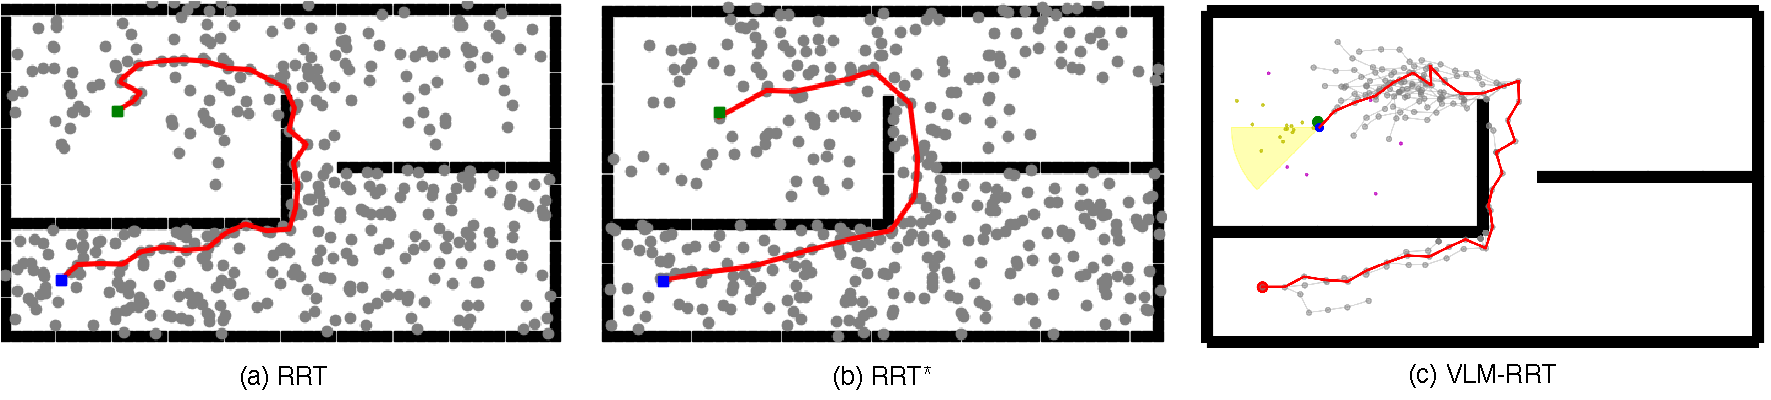
\includegraphics[width=1.0\textwidth]{images/Baseline.pdf}
    \caption{Illustrative example of the path-planning behavior obtained with: (a) RRT, (b) RRT* and (c) VLM-RRT.}
    \label{fig:Baseline_image}
\end{figure*}
%%%%%%%%%%%%%%%%%%%%%%%%%%%%%%%%%%%%%%%% Baseline %%%%%%%%%%%%%%%%%%%%%%%%%%%%%%%%%%%%%%%%%%%%%%%

\subsection{Simulation Setup} 
\label{ssec:sim_setup}
%To evaluate our approach, we assume that an autonomous UAV agent evolves (assuming a fixed altitude) inside a bounded environment $\mathcal{E} \subset \mathbb{R}^2$ of dimensions $500$m $\times$ $500$m. The agent's its planar motion is captured by a 4-dimensional state vector \( x(t) = [x_1, x_2, \dot{x}_1, \dot{x}_2]^\top \in \mathcal{X} \subset \mathbb{R}^4 \) comprising of its position $(x_1,x_2) \in \mathbb{R}^2$ and velocity $(\dot{x}_1,\dot{x}_2) \in \mathbb{R}^2$ components within the 2D Cartesian coordinate system. The agent is controllable, and capable of following specific directional and speed commands via the control input $u(t) \in \mathcal{U} \subset \mathbb{R}^2$, which corresponds to the applied control force. The matrices $A \in \mathbb{R}^{4\times4}$ and $B \in \mathbb{R}^{4\times2}$ shown in Eq. \eqref{eq:LTI} are given by:
%\begin{equation*}
%A = 
%\begin{bmatrix}
%    I_{2\times2} & \Delta T \cdot I_{2\times2}\\
%    0_{2\times2} & (1-\zeta) \cdot I_{2\times2}
%\end{bmatrix},~ B = 
%\begin{bmatrix}
%    0_{2\times2} \\
%    \frac{\Delta T}{m} \cdot I_{2\times2}
%\end{bmatrix},
%\end{equation*}
%
%\noindent where $\Delta T$ signifies the sampling interval, $\zeta$ is the air resistance coefficient, and $m$ represents the mass of the agent. Additionally, $I_{2\times2}$ and $0_{2\times2}$ are the 2-by-2 identity and zero matrices, respectively. The output vector $y(t) \in \mathcal{Y} \subset \mathbb{R}^2$ consists of the UAV's position at time step $t$, therefore the matrices $C\in \mathbb{R}^{2\times4}$ and $D\in \mathbb{R}^{2\times2}$ are given by $\left[ \begin{smallmatrix} I_{2\times2} & 0_{2\times2}\end{smallmatrix} \right]$ and $0_{2\times2}$ respectively. The parameters $\Delta T$, $\zeta$, and $m$ are set to 1s, 0.2, and 1.05kg respectively. The control input is bounded in each dimension in the range $[-10, 10]$N, and the UAV's maximum velocity is capped at $v_\text{max}=15$m/s. The staring and goal regions $\mathcal{S}$ and $\mathcal{G}$, as well as the fire fronts to be avoided $o \in \mathcal{O}$ are  represented rectangular regions with random dimensions as shown in Fig.\ref{fig:system_achitecture}(a). 
%
%Unless otherwise indicated the VLM-RRT step size $\delta$ is set to $\Delta T \cdot v_\text{max}$ and $\epsilon=1$m. The sampling sector $\mathcal{R}$ has radius $r=30$m, and $\theta=45$deg, and the default value for the probability $\gamma$ is set to $0.85$.
%We should mention here that the output of the VLM-RRT algorithm is a path of length $\ell$ i.e., a sequence of $\ell$ points, and is converted to the continuous reference path $\mathcal{P}$ to be tracked by fitting a spline curve \cite{wang2002arc}. The planning horizon is set to $T=2.5\ell$, and subsequently $T$ evenly spaced points (i.e., equal arc-length spacing) are sampled from $\mathcal{P}$ between the staring and goal points. The optimization in Eq. \eqref{eq:MPC} is solved as a quadratic program (QP) with the Gurobi solver, with the matrices $Q$ and $R$ set to $0.9I_{2 \times 2}$, and $0.1I_{2 \times 2}$ respectively.
%
%We have evaluated the performance of our proposed approach by integrating two state-of-the-art VLMs to support autonomous navigation: OpenAI's GPT-4o \cite{achiam2023gpt} and Meta's Llama 3.2 90B Vision Instruct \cite{dubey2024llama}. GPT-4o is a multi-modal model with approximately 1.8 trillion parameters, accessed via OpenAI's API, whose advanced vision-language processing capabilities were leveraged for environmental interpretation and decision support within our UAV navigation framework. In contrast, Meta's Llama 3.2 90B Vision Instruct, with 90 billion parameters, facilitates multimodal reasoning to provide visual understanding and contextual analysis critical to the VLM-RRT path planning algorithm. 

%For both models, inputs were configured to include environmental snapshots and corresponding textual prompts. The integration of these VLMs enhanced spatial reasoning and enabled more robust interpretation of environmental contexts, thereby strengthening the decision-making process for autonomous UAV navigation.




To evaluate our approach, we assume that an autonomous UAV agent evolves (assuming a fixed altitude) inside a bounded environment \( \mathcal{E} \subset \mathbb{R}^2 \) of dimensions \( 500 \, \text{m} \times 500 \, \text{m} \). The agent's planar motion is captured by a 4-dimensional state vector \( x(t) = [x_1, x_2, \dot{x}_1, \dot{x}_2]^\top \in \mathcal{X} \subset \mathbb{R}^4 \), comprising its position \( (x_1, x_2) \in \mathbb{R}^2 \) and velocity \( (\dot{x}_1, \dot{x}_2) \in \mathbb{R}^2 \) components within the 2D Cartesian coordinate system. The agent is controllable and capable of following specific directional and speed commands via the control input \( u(t) \in \mathcal{U} \subset \mathbb{R}^2 \), which corresponds to the applied control force. The matrices \( A \in \mathbb{R}^{4 \times 4} \) and \( B \in \mathbb{R}^{4 \times 2} \), shown in Eq.~\eqref{eq:LTI}, are given by:
\begin{equation*}
A = 
\begin{bmatrix}
    I_{2 \times 2} & \Delta T \cdot I_{2 \times 2} \\
    0_{2 \times 2} & (1 - \zeta) \cdot I_{2 \times 2}
\end{bmatrix}, \quad B = 
\begin{bmatrix}
    0_{2 \times 2} \\
    \frac{\Delta T}{m} \cdot I_{2 \times 2}
\end{bmatrix},
\end{equation*}
where \( \Delta T \) signifies the sampling interval, \( \zeta \) is the air resistance coefficient, and \( m \) represents the mass of the agent. Additionally, \( I_{2 \times 2} \) and \( 0_{2 \times 2} \) are the 2-by-2 identity and zero matrices, respectively. The output vector \( y(t) \in \mathcal{Y} \subset \mathbb{R}^2 \) consists of the UAV's position at time step \( t \); therefore, the matrices \( C \in \mathbb{R}^{2 \times 4} \) and \( D \in \mathbb{R}^{2 \times 2} \) are given by \( \begin{bmatrix} I_{2 \times 2} & 0_{2 \times 2} \end{bmatrix} \) and \( 0_{2 \times 2} \), respectively. The parameters \( \Delta T \), \( \zeta \), and \( m \) are set to \( 1 \, \text{s} \), \( 0.2 \), and \( 1.05 \, \text{kg} \), respectively. The control input is bounded in each dimension within the range \( [-10, 10] \, \text{N} \), and the UAV's maximum velocity is capped at \( v_{\text{max}} = 15 \, \text{m/s} \). The starting and goal regions \( \mathcal{S} \) and \( \mathcal{G} \), as well as the fire fronts to be avoided \( o \in \mathcal{O} \), are represented as rectangular regions with random dimensions, as shown in Fig.~\ref{fig:system_achitecture}(a).

Unless otherwise indicated, the VLM-RRT step size \( \delta \) is set to \( \Delta T \cdot v_{\text{max}} \) and \( \epsilon = 1 \, \text{m} \). The sampling sector \( \mathcal{R} \) has radius \( r = 30 \, \text{m} \) and angle \( \theta = 45^\circ \), and the default value for the probability \( \gamma \) is set to \( 0.85 \). We should mention here that the output of the VLM-RRT algorithm is a path of length \( \ell \), i.e., a sequence of \( \ell \) points, which is converted to the continuous reference path \( \mathcal{P} \) to be tracked by fitting a spline curve~\cite{wang2002arc}. The planning horizon is set to \( T = 2.5\ell \), and subsequently, \( T \) evenly spaced points (i.e., with equal arc-length spacing) are sampled from \( \mathcal{P} \) between the starting and goal points. The optimization in Eq.~\eqref{eq:MPC} is solved as a quadratic program (QP) with the Gurobi solver, with the matrices \( Q \) and \( R \) set to \( 0.9 I_{2 \times 2} \) and \( 0.1 I_{2 \times 2} \), respectively.

We have evaluated the performance of our proposed approach by integrating two state-of-the-art VLMs to support autonomous navigation: OpenAI's GPT-4o~\cite{achiam2023gpt} and Meta's Llama 3.2 90B Vision Instruct~\cite{dubey2024llama}. GPT-4o is a multimodal model with approximately 1.8 trillion parameters, accessed via OpenAI's API, whose advanced vision-language processing capabilities were leveraged for environmental interpretation and decision support within our UAV navigation framework. In contrast, Meta's Llama 3.2 90B Vision Instruct, with 90 billion parameters, facilitates multimodal reasoning to provide visual understanding and contextual analysis critical to the VLM-RRT path-planning algorithm.

%%%%%%%%%%%%%%%%%%%%%%%%%%%%%%%%%%%%%%%% Baseline %%%%%%%%%%%%%%%%%%%%%%%%%%%%%%%%%%%%%%%%%%%%%%%
\begin{table}
\centering
\caption{Performance Comparison with Competing Approaches.}
\resizebox{\columnwidth}{!}{ % Adjusts the table width to fit the column
\begin{tabular}{l c c c}
\hline
\textbf{Algorithm} & \textbf{LLM} & \textbf{Avg. Iterations ($N$)} & \textbf{Avg. Path Length (m)} \\
\hline
\addlinespace
A* \cite{Hart1968}       & -         & 514 & 52.73 \\
\addlinespace
\multirow{2}{*}{LLM-A* \cite{meng2024llm}} & GPT-4o     & 410 & 52.73 \\
                        & Llama 3.2V & 405 & 52.80 \\
\hline
\addlinespace
RRT      & -         & 423 & 56.48 \\
RRT* \cite{karaman2011sampling}    & -         & 477 & 53.89 \\
\addlinespace
\multirow{2}{*}{VLM-RRT} & GPT-4o     & 172  & 54.56 \\
                        & Llama 3.2V & 176  & 55.87 \\
\hline
\end{tabular}
}
\label{tab:Baseline_table}
% \vspace{5pt} % Adjust space before the note
% \begin{minipage}{\linewidth}
% \centering
% \small \textit{Note: CoT prompt technique is used in above experiments}
% \end{minipage}
\end{table}
%%%%%%%%%%%%%%%%%%%%%%%%%%%%%%%%%%%%%%%% Baseline %%%%%%%%%%%%%%%%%%%%%%%%%%%%%%%%%%%%%%%%%%%%%%

%%%%%%%%%%%%%%%%%%%%%%%%%%%%%%%%%%%%%%%% VLM-RRT %%%%%%%%%%%%%%%%%%%%%%%%%%%%%%%%%%%%%%%%%%%%%%%
\begin{table*}[t]
\centering
\caption{Performance of VLM-RRT under various models and prompting techniques.}
\resizebox{\textwidth}{!}{ % Adjusts the table width to fit the column
% \renewcommand{\arraystretch}{1.2} % Adjust row height for better readability
\begin{tabular*}{\textwidth}{@{\extracolsep{\fill}} l c c c c c}
\hline
\textbf{Algorithm} & \textbf{VLM} & \textbf{Prompt Technique} & \textbf{Success Rate} & \textbf{Avg. Iterations ($N$)} & \textbf{Avg. Path Length (m)} \\
\hline
\addlinespace
RRT  & - & - & 82\% (41/50) & 343 & 58 \\
RRT* & - & - & 88\% (44/50) & 302 & 45 \\
\midrule
\multirow{3}{*}{VLM-RRT (Ours)} & \multirow{3}{*}{GPT-4o} & Zero-shot & 68\% (34/50) & 93 & 47 \\
 & & Few-shot & 94\% (47/50) & 89 & 46 \\
 & & CoT      & 86\% (43/50) & 94 & 48 \\
\cmidrule{2-6}
 & \multirow{3}{*}{Llama 3.2V} & Zero-shot & 56\% (28/50) & 102 & 48 \\
 & & Few-shot  & 90\% (45/50) & 88 & 49 \\
 & & CoT       & 78\% (39/50) & 95 & 47 \\
\hline
\end{tabular*}
}
\label{tab:VLM-RRT_Table}
\end{table*}
%%%%%%%%%%%%%%%%%%%%%%%%%%%%%%%%%%%%%%%% VLM-RRT %%%%%%%%%%%%%%%%%%%%%%%%%%%%%%%%%%%%%%%%%%%%%%%



\subsection{Results}

We begin the evaluation by comparing the proposed approach with the closely related work in~\cite{meng2024llm}, where the authors integrated LLMs with the A* path-finding algorithm~\cite{Hart1968}. Additionally, we compare it with the traditional RRT approach~\cite{lavalle1998rapidly} and the RRT* algorithm~\cite{karaman2011sampling}. Table~I presents the average number of iterations required for convergence and the resulting path length for each approach. These results were obtained by averaging 100 random scenarios (i.e., random environment configurations) in a Monte Carlo (MC) simulation.
It is important to note that while the A* and RRT approaches are not directly comparable (in terms of the number of iterations), the results indicate a consensus on the performance improvement achieved when these planning algorithms are integrated with LLMs. In particular, the VLM-RRT approach significantly improves the convergence rate compared to the original RRT algorithm while also enhancing path quality (in terms of path length). Moreover, the VLM-RRT approach achieves path quality comparable to that of the more advanced RRT*, but with fewer iterations. An illustrative example is shown in Fig.~\ref{fig:Baseline_image}. These results were obtained using CoT prompting.


%%%%%%%%%%%%%%%%%%%%%%%%%%%%%%%%%%%% Dynamic Location %%%%%%%%%%%%%%%%%%%%%%%%%%%%%%%%%%%%%%%%%
\begin{figure*}
    \centering
    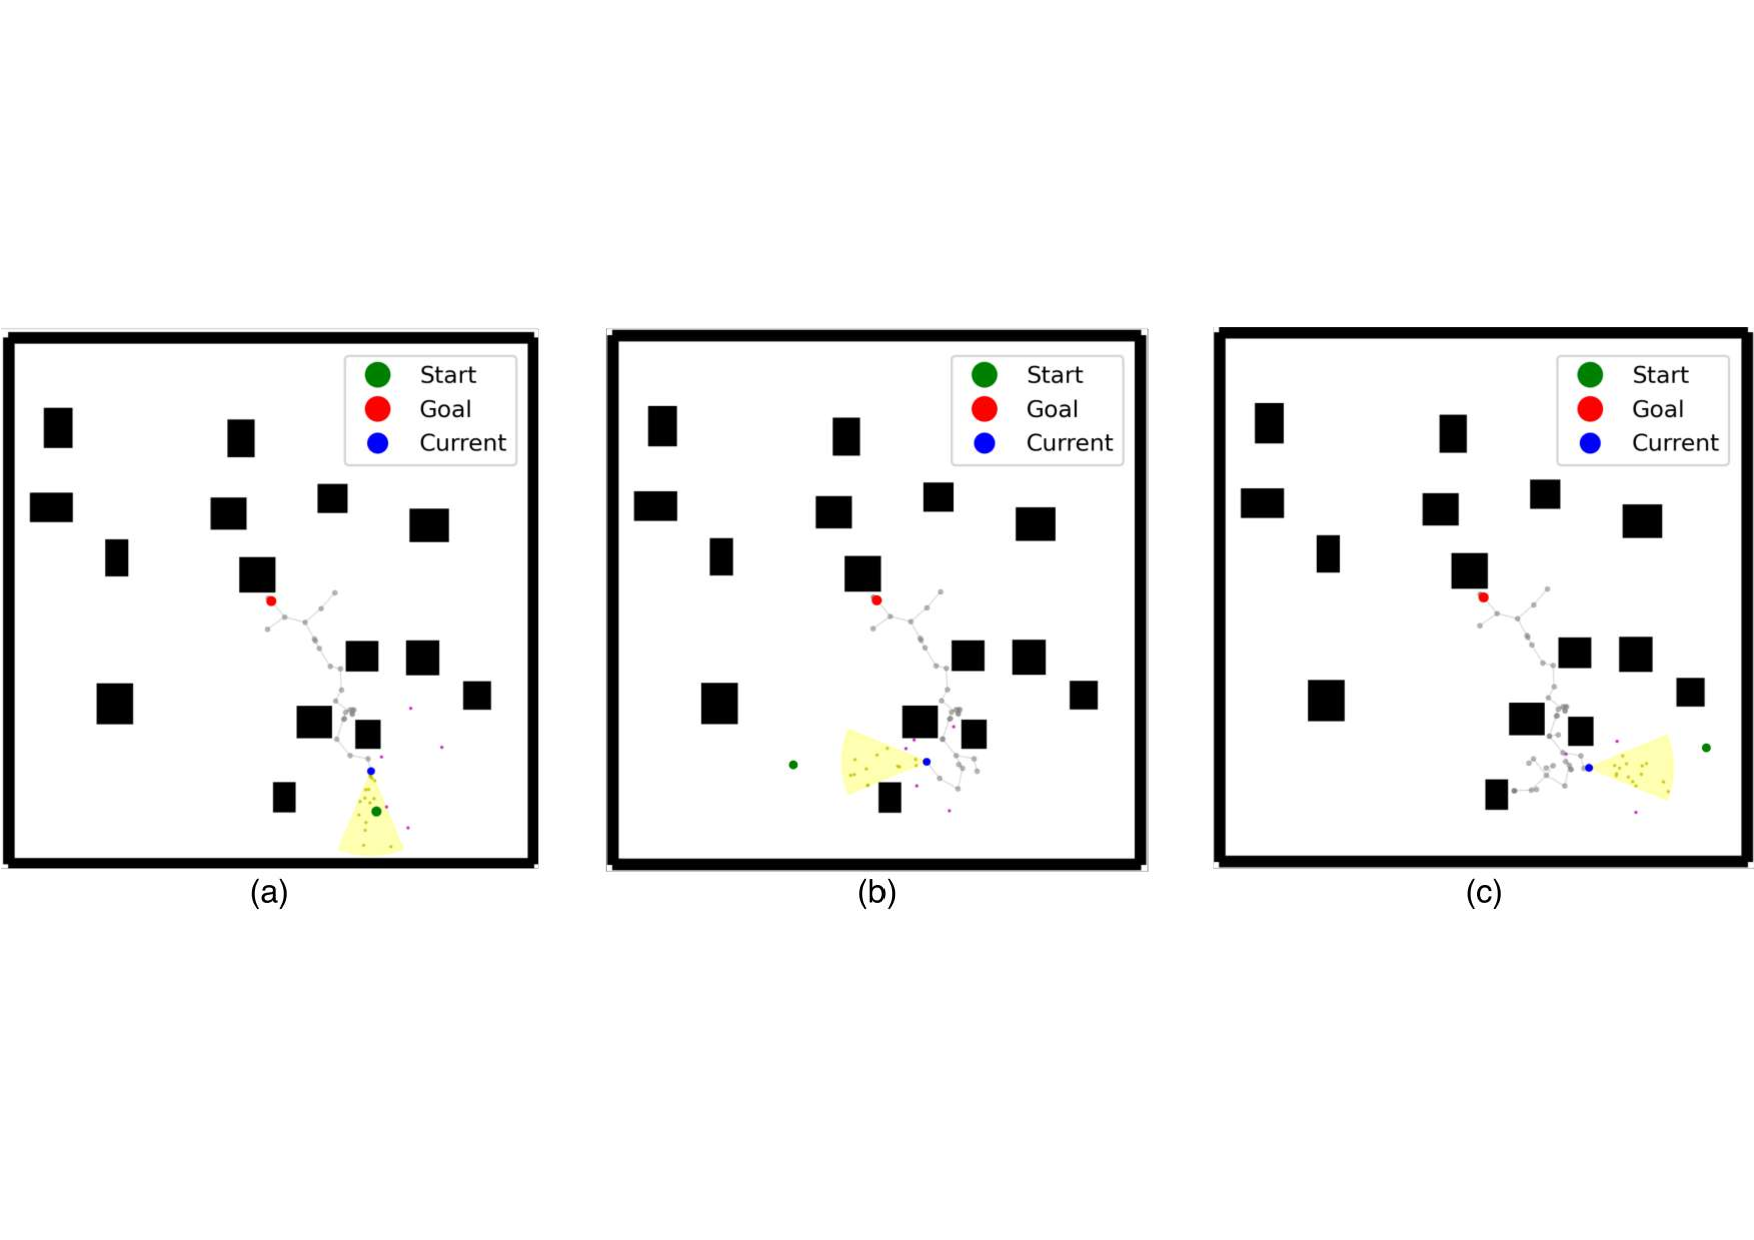
\includegraphics[width=1.0\textwidth]{images/dynamic_location.pdf}
    \caption{Illustration of the VLM-RRT algorithm navigating toward dynamic goals in a 2D environment. The scenario involves three goal relocations. Red point is the starting position, green point is the goal position which  changes over time, and the blue point is a leaf node. The yellow sector is the VLM-informed sampling region.}
    \label{fig:dynamic_location}
\end{figure*}
%%%%%%%%%%%%%%%%%%%%%%%%%%%%%%%%%%%% Dynamic Location %%%%%%%%%%%%%%%%%%%%%%%%%%%%%%%%%%%%%%%%%

In the next experiment, we conduct a more thorough analysis of the proposed VLM-RRT approach in terms of the following metrics:
\begin{enumerate}
    \item \textbf{Success Rate:} Defined as the percentage of experiments in which a collision-free path from the start to the goal region is successfully found within the maximum number of iterations \( N = 500 \).
    \item \textbf{Number of Iterations:} The total number of iterations required to obtain a feasible path.
    \item \textbf{Path Length:} Assessed via the length of the final path from the start to the goal region.
\end{enumerate}
The above metrics are computed on a per-experiment basis and then averaged across 250 MC runs, as shown in Table~II. As shown in the results, RRT and RRT* achieve success rates of 82\% and 88\%, respectively. In contrast, VLM-RRT surpasses the performance of the traditional approaches, particularly under few-shot and CoT prompting, while requiring significantly fewer iterations. Additionally, VLM-RRT achieves higher path quality in terms of path length compared to the traditional RRT, as shown in Table~II. In terms of path length, VLM-RRT achieves performance comparable to the more advanced RRT*, though this is accomplished with fewer iterations. The results also highlight the differences in performance obtained using different prompting techniques, as well as the effectiveness of the two LLMs, indicating an advantage for GPT-4o.



%%%%%%%%%%%%%%%%%%%%%%%%%%%%%%%%%%%%% Sampling Distribution %%%%%%%%%%%%%%%%%%%%%%%%%%%%%%%%%%%
\begin{table}
\centering
\caption{VLM-RRT robustness analysis}
\resizebox{\columnwidth}{!}{ % Adjusts the table width to fit the column
\begin{tabular}{c c c}
\hline
\boldmath{$\gamma$} & \textbf{Success Rate (\%)} & \textbf{Avg. Number of Iterations ($N$)} \\
\hline
1.0  & 79  & 86 \\
0.9  & 88  & 92 \\
0.8  & 92 & 105 \\
0.7  & 95  & 102 \\
0.6  & 93  & 128 \\
0.5  & 89  & 142 \\
\hline
\end{tabular}
}
\label{tab:sampling_results}
\end{table}
%%%%%%%%%%%%%%%%%%%%%%%%%%%%%%%%%%%%% Sampling Distribution %%%%%%%%%%%%%%%%%%%%%%%%%%%%%%%%%%%

The next experiment investigates how the parameter \( \gamma \) (i.e., the probability of taking a VLM-informed decision) affects the sensitivity of the algorithm and how this can be fine-tuned to increase the robustness of VLM-RRT. Table~\ref{tab:sampling_results} shows the algorithm's performance (in terms of success rate and number of iterations) for different values of \( \gamma \) ranging from 1 to 0.5, obtained over 100 MC trials. When \( \gamma = 1 \), VLM-RRT always takes a VLM-informed decision at each time step and samples a new point from within the area suggested by the VLM. Although this can lead to faster convergence in many situations, the results show that this strategy decreases robustness (i.e., increases the likelihood of failure to converge). From our experiments, we have observed that this is due to two main reasons: (a) the VLM can make mistakes, which consequently lead the algorithm to make incorrect decisions, and (b) \( \gamma = 1 \) leads to greedy behavior, which in turn causes the algorithm to become stuck in infeasible regions. On the other hand, a lower value of \( \gamma \) causes the algorithm to behave more similarly to the original RRT, resulting in a drop in success rate due to reaching the maximum number of iterations. Therefore, a fine-tuned value of \( \gamma \) optimally balances exploration and exploitation, leading to enhanced robustness and performance, as shown.

In emergency response scenarios, mission parameters often change dynamically as new information becomes available. For instance, the location of survivors may be updated based on new sensor data or witness reports, requiring rapid replanning of UAV trajectories. To evaluate our system's performance in such dynamic scenarios, we conducted a series of experiments with dynamic goal locations. Figure~\ref{fig:dynamic_location} shows one such scenario where the goal region changes location dynamically during the mission.
The VLM demonstrated a consistent ability to identify changes in the location of the goal region during the mission, achieving a detection rate of 92\% across 50 random scenarios in which the goal region's location varied over time. In cases where the VLM failed to immediately recognize the new goal location, it typically required one additional sampling iteration to correct its direction.
We observed that the VLM's performance in recognizing and adapting to new goal locations remained robust even in cluttered environments, though the convergence time increased when obstacles were present between the UAV's position and the new goal location. This increase in convergence time was primarily due to the necessary local path adjustments around obstacles rather than any delay in goal recognition or sampling direction updates.















%%%%%%%%%%%%%%%%%%%%%%%%%%%%%%%%%%%%% Section 5: Evaluation %%%%%%%%%%%%%%%%%%%%%%%%%%%%%%%%%%%%